%\documentclass[10pt,handout]{beamer}
\documentclass[10pt]{beamer}
\usepackage{babel} % Anpassa efter svenska. Ger svensk logga.
\usepackage[utf8]{inputenc} % Anpassa efter linux
\usepackage{graphicx}
\usepackage{../common/beamerthemeUppsala}
%\usecolortheme{UU} % Anpassa efter UU:s frger och logga
%\hypersetup{pdfpagemode=FullScreen} % Adobe Reader ska ppna fullskrm
\setbeamertemplate{itemize items}[circle]

% \usepackage{beamerthemesplit}
\usepackage{amsmath}
\usepackage{amssymb}
% \usepackage{graphics}
% \usepackage{graphicx}
% \usepackage{epsfig}
% \usepackage[latin1]{inputenc}
 \usepackage{color}
% \usepackage{fancybox}
% \usepackage{psfrag}
% \usepackage[english]{babel}
 \setbeamertemplate{footline}{\hfill\insertframenumber/\inserttotalframenumber}


% Read in commands
% Course settings
\newcommand{\currentsemester}{Autumn 2024}

% New commands
\newcommand{\bfm}[1]   {\mbox{\boldmath{${#1}$}}}
\newcommand{\Prob}   {\mbox{\textnormal{P}}}
\newcommand{\uured}[1]{\textcolor{uured}{#1}}

% Eqds
\def\eqd{\,{\buildrel d \over =}\,}

% Math operators
\DeclareMathOperator{\E}{\mathbb{E}}
\DeclareMathOperator{\V}{\mathbb{V}}



%%%%%%%%%%%%%%%%%%%%%%%%%%%%%%%%%%%%%%%%%%%%%%%%%%%%%%%%%%%%%%%%%%

\setlength{\parskip}{3mm}
\title[]{{\color{black}Machine learning -- Large Language Models}}
\author[]{M{\aa}ns Magnusson\\Department of Statistics, Uppsala University}
\date{\currentsemester}


\begin{document}

\frame{\titlepage
% \thispagestyle{empty}
}

%%%%%%%%%%%%%%%%%%%%%%%%%%%%%%%%%%%%%%%%%%%%%%%%%%%%%%%%%%%%%%%%%%




\section{Introduction} % to Large Language Models

\begin{frame}{What is a Large Language Model?}

\begin{itemize}
  \item Large Language Models (LLM) are commonly defined as:
  \begin{itemize}
      \item large natural language models (usually transformer-based)
      \pause
      \item generative and autoregressive, predicting a token at a time, based on previous \uured{context}
      \pause
      \item having some ability to achieve \uured{general-purpose language "understanding"}
      \item show \uured{emergent} abilities to solve other more complex tasks
      \pause
      \item fit for few-shot learning and \uured{incontext} learning
      \pause
      \item pre-trained on very large data
  \end{itemize}
  \item Compared to pretrained language models (PLM), LLMs are
  \begin{itemize}
      \item larger (billions or trillions, rather than millions of parameters), in practice only possible to train by a few persons
      \item possible to use for in-context learning
      \item usually interacted with through the prompt
  \end{itemize}
\end{itemize}

\end{frame}

\begin{frame}{Historical development}

\begin{figure}[h]
\centering
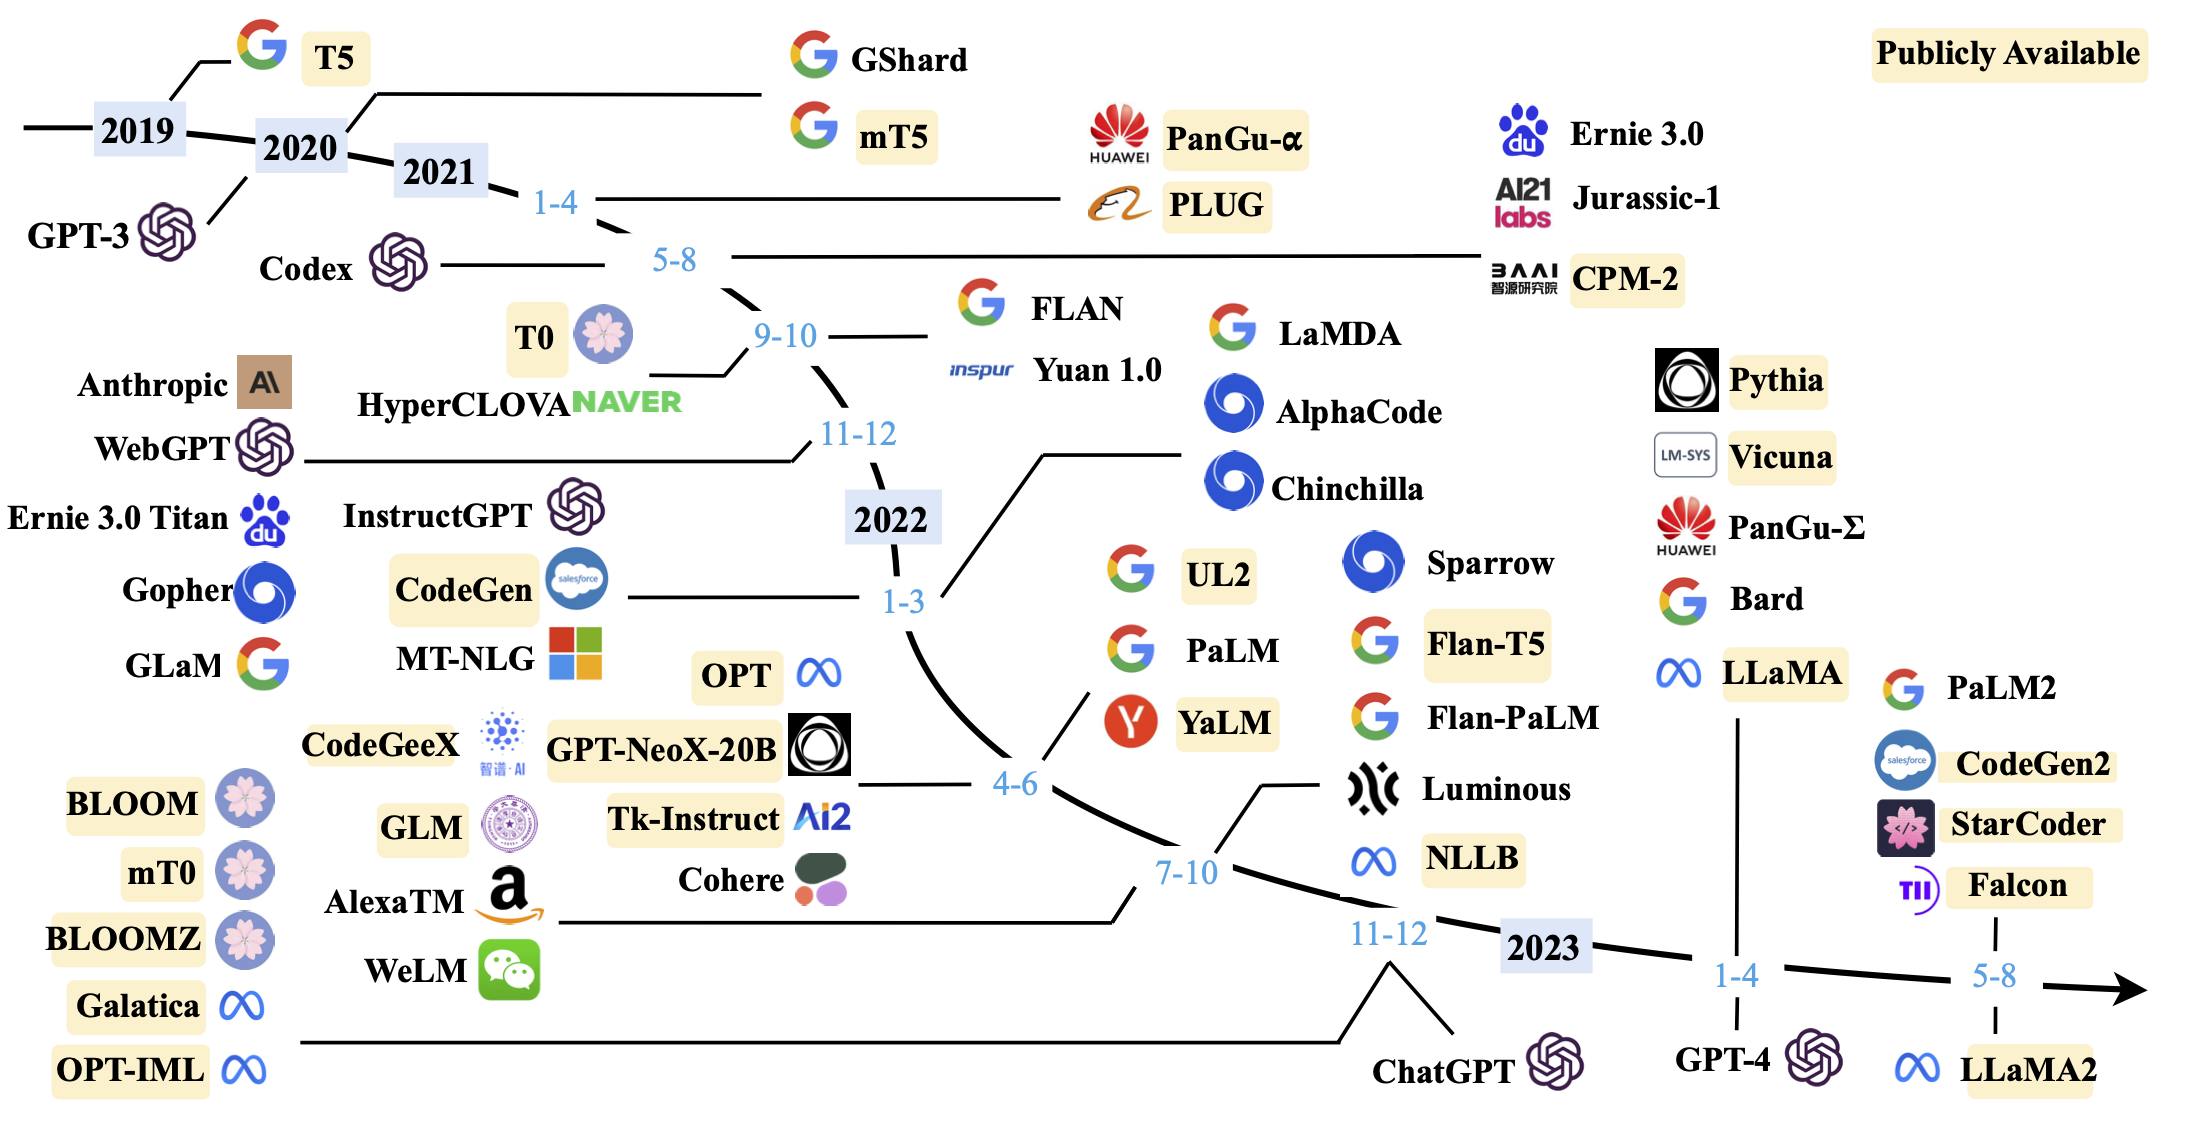
\includegraphics[width=0.99\textwidth]{fig/fig2_zhao_2023}
\caption{The development of LLMs (Figure 2, Zhao et al., 2023)}
\end{figure}

\begin{itemize}
    \item Milestones (subjective): GPT-3, GPT-4, chatGPT, Llama 2
\end{itemize}

\end{frame}

\begin{frame}{A subset of current LLMs}

\begin{figure}[h]
\centering
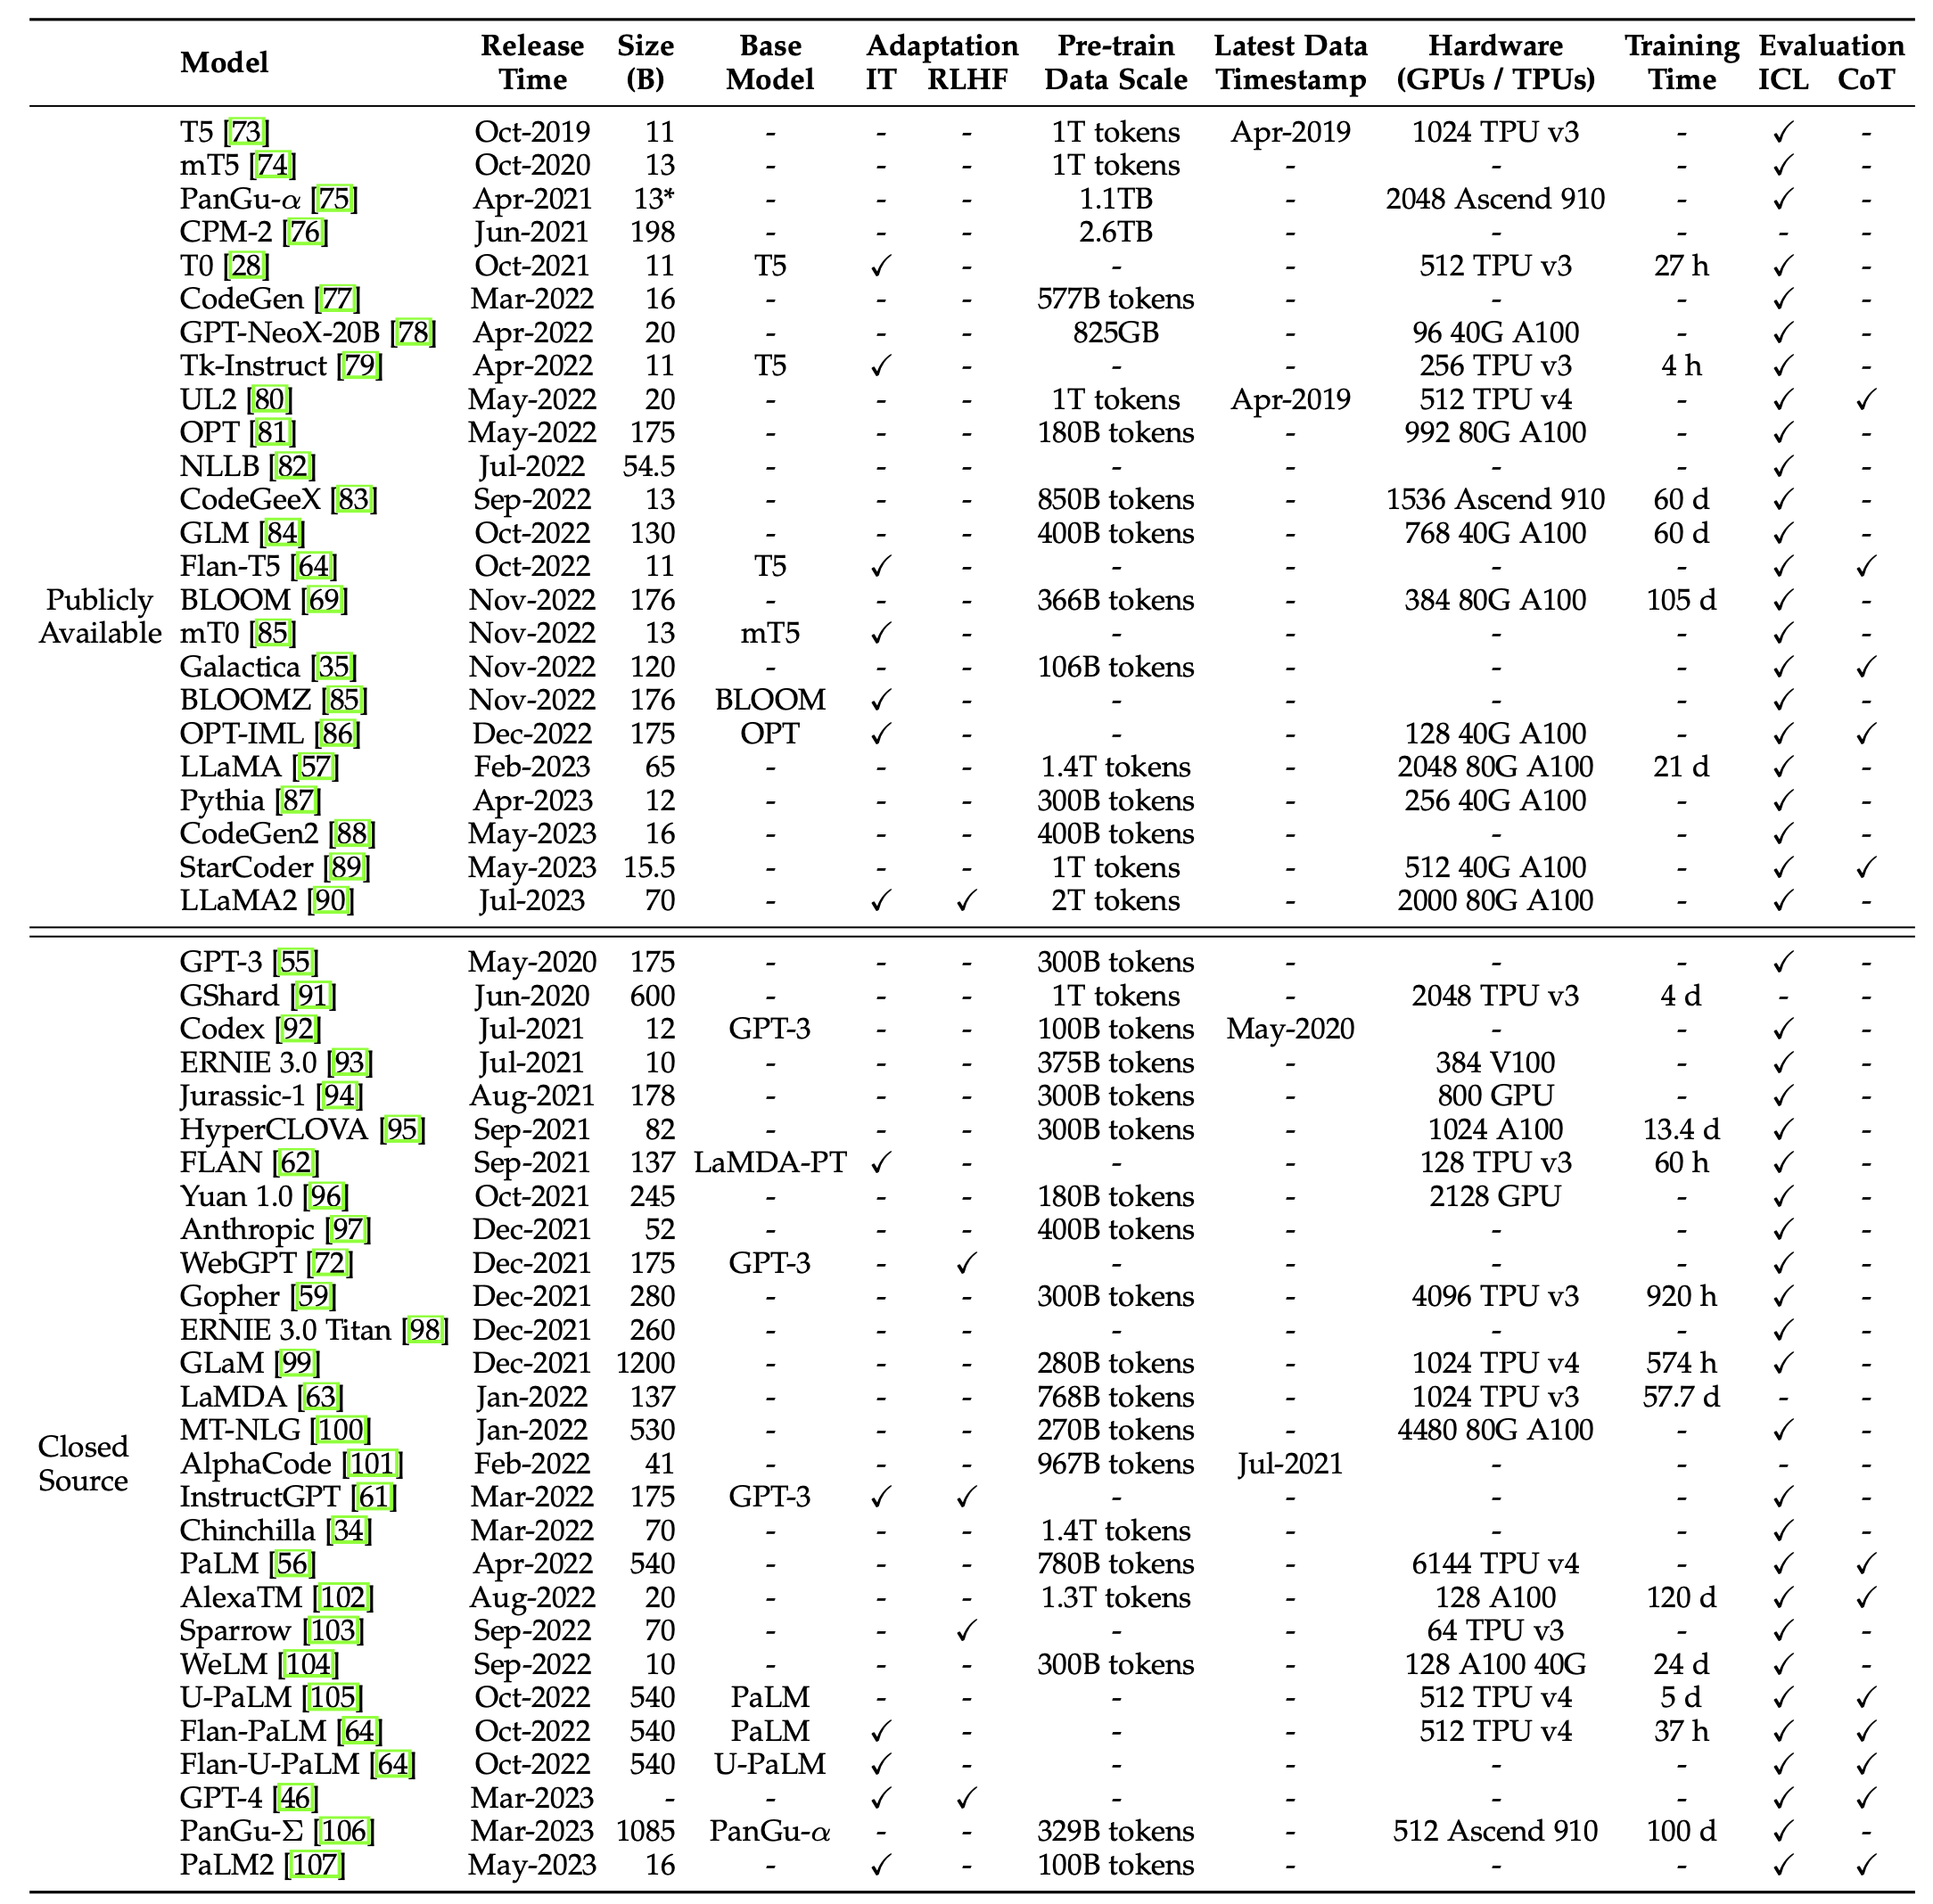
\includegraphics[width=0.82\textwidth]{fig/tab1_zhao_2023}
\caption{Statistics of LLMs (Table 1, Zhao et al., 2023)}
\end{figure}

\end{frame}

\begin{frame}{Examples of LLM prompting}

Examples:
\begin{enumerate}
\item Can you please add 113329 and 719292? (true is 832621)
\item Who is Olof Palme? Please respond both in English and Swedish.
\end{enumerate}

\centering

\vspace{5mm}

\href{https://www.llama2.ai/}{Llama 2}

\vspace{10mm}

\href{https://chat.openai.com/}{chatGPT}

\end{frame}


\begin{frame}{Why is this working now?}

\begin{itemize}
\item Scaling of pretrained models, performals (loss) improves by:
\begin{itemize}
\item Larger models (GPT3 175B, PaLM 540B)
\item Larger datasets
\item More computation
\item Scaling laws (CITE, CITE) show that all three are important\\
\uured{Can we connect this back to the standard ML framework?}
% Scaling laws has shown that all three matters and is of importance.
\end{itemize}
\pause
\item Fine-tuning for tuning models to follow instructions (InstructGPT)
\end{itemize}

\end{frame}


%\begin{frame}{Scaling laws}

%Extensive research has shown that scaling can largely improve the model capacity of LLMs

% Scale Matters/ Scaling laws p 4 in Zhao
% model performance with respective to three major factors
% namely model size (N), dataset size (D),

%\end{frame}


\begin{frame}{Emergant abilities}
% Emergent abilities
% p 4 in Zhao
\begin{itemize}
\item "the abilities that are not present in small models but arise in large models" (Zhao et al, 2023)
\item One of the main differences between LLMs and PLMs
\item Examples:
\begin{itemize}
\item In-context learning (basis for prompting)
\item Instruction following % "LaMDA-PT started to significantly outperform the untuned one on unseen tasks when the model size reached 68B, but not for 8B or smaller model sizes."
\item Step-by-step reasoning
\end{itemize}
\end{itemize}



\end{frame}


\begin{frame}{In-context learning (ICL)}

\begin{itemize}
\item Learning tasks in the actual context (think chat).
\item We demonstrate what to do with a few examples
\item The model learn what todo \uured{in context}
\item ICL only prompts LLMs for utilization
\item Let
\[
D_k = \left(f(x_1, y_1),...,f(x_k, y_k) \right)
\]
then
\[
\hat{y} = \text{LLM}(I, \underbrace{\left(f(x_1, y_1),...,f(x_k, y_k)\right)}_{demonstrations}, \underbrace{f(x_{k+1}}_{input} , ...)
\]
where $I$ is the general instructions.
\item The problem is to design the instructions in a good way.
\item What happens under the hood? We position the model in embeddings space.
\item Crazy examples: "Take a deep breath and think hard."
\item Several studies have shown that the effectiveness of ICL is highly affected by the design of demonstrations %[350, 370, 371]

\end{itemize}

% TODO: A comprehensive review of ICL has been presented in the survey paper [50], and we suggest the readers refer- ring to it for a more general, detailed discussion on this topic.
% In-context learning
% 6.1 Zhao

\end{frame}


\begin{frame}{Demonstration}
% Zhao see 6.1.2.
% the selected demon- stration examples in ICL should contain sufficient informa- tion about the task to solve as well as be relevant to the test query, for the above two selection approaches.

\begin{itemize}
\item  Demonstration selection
\begin{itemize}
\item Not well explored: k-NN based retriever to select examples
\item To resolve this issue, diversity-based selection strategies are proposed to choose the most representative set of examples for specific tasks
\item LLM-based methods to choose examples. E.g. ome recent studies employ LLM itself as the demonstration generator without human intervention
\end{itemize}
\item Demonstration format
\begin{itemize}
\item "Lets think step by step", "Take a deep breath and think."
\end{itemize}
\item Demonstration order
\begin{itemize}
\item Indications of recency bias (they are prone to repeat answers that are near the end of demonstrations)
\item Why?
\end{itemize}

\end{itemize}


\end{frame}




\begin{frame}{Chain of thought (CoT) prompting}

% Zhao Section 6.2

\begin{itemize}
\item Prompting strategy to improve performance in "reasoning"
\item Incorporates intermediate reasoning steps that can lead to the final output
\item instead of (input, output), we use (input, cot, output)
\item Zero-shot CoT: "Lets think step by step"
\end{itemize}

\begin{figure}[h]
\centering
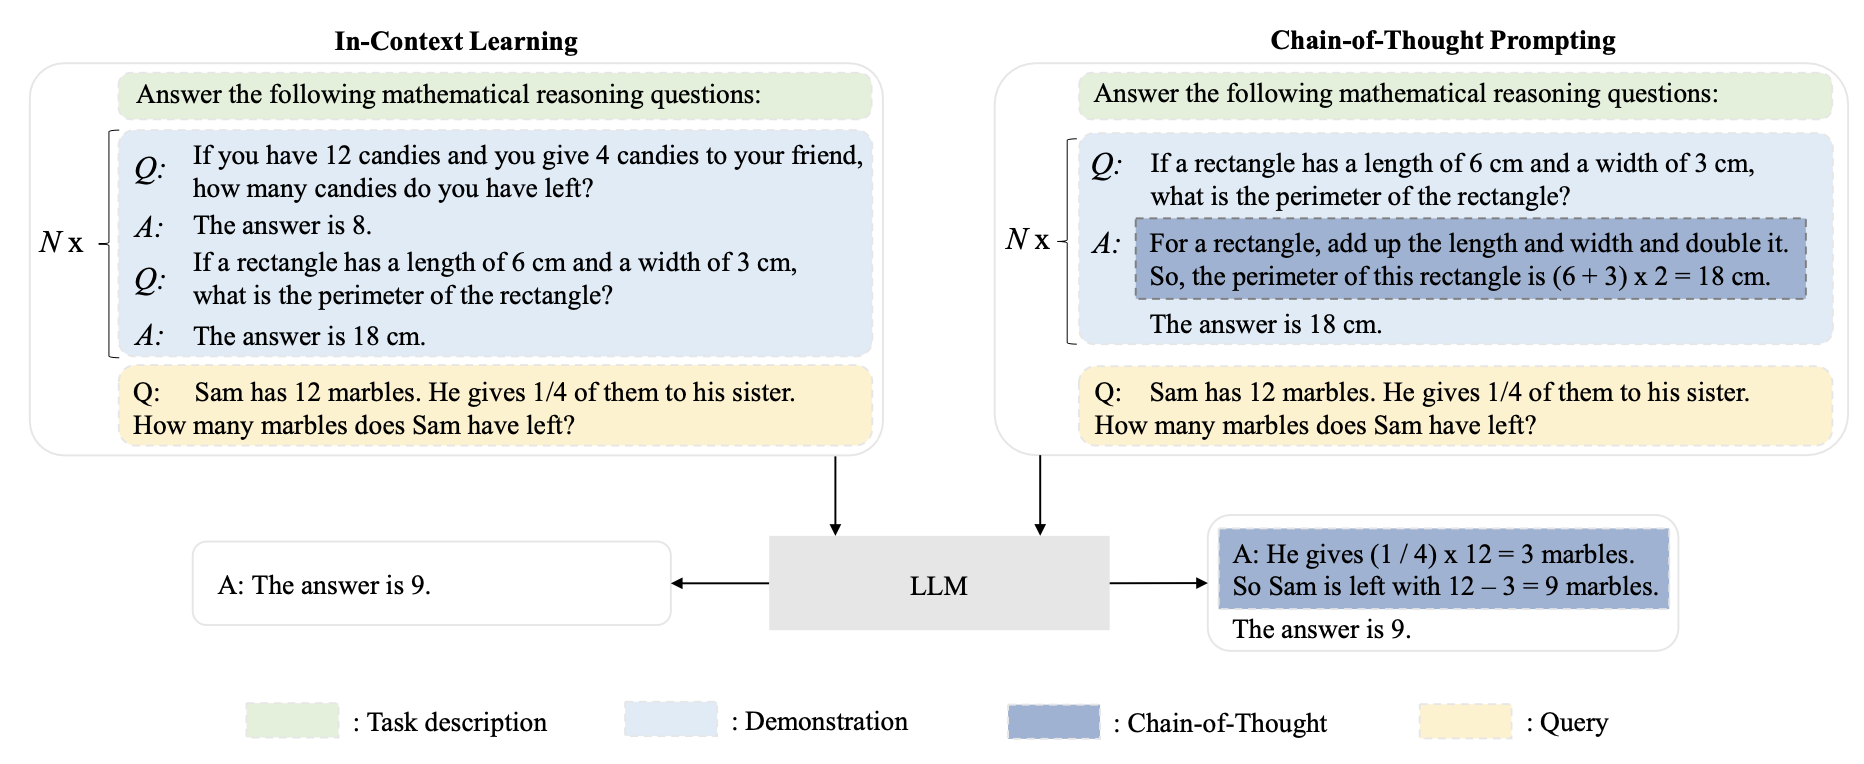
\includegraphics[width=0.99\textwidth]{fig/zhao_2023_fig12}
\caption{ICL vs CoT (Figure 12, Zhao et al., 2023)}
\end{figure}

\end{frame}

\begin{frame}{Instruction tuning/following}

% instruction tuning (discussed in Section 5.1)

\end{frame}


\begin{frame}{Alignments}

% Aligning p 4 in Zhao
% RLHF

\end{frame}


\begin{frame}{Hallucinations}

% Zhao
% Hallucinations
% Kaddour (2023): 2.8, Fig 7


%
% Hallucinations

\end{frame}

\section{Architectures}

\begin{frame}{GPT-3}


\end{frame}

\begin{frame}{GPT-3.5/4}


\end{frame}

\begin{frame}{Llama 2}


\end{frame}


\begin{frame}{Others}

% Table

\end{frame}


\begin{frame}{Parameters and Model Size}

% Parameters and Model Size: Use Table 1

% Uset table 3 here from Zhao


\end{frame}


\begin{frame}{Decoding (word generation)}

% Decoding (4.2.4) - sampling and temperature sampling


\end{frame}



\section{Training}

\begin{frame}{(Pre-training) Data}

% 1. Data Collection
% use Table 2 Zhao p 11 and part 4.1
% Use Figure 5 here
% Quality filtering: p 14

\end{frame}

\begin{frame}{Huge Data}

% Kaddour (2023): Unfathomable datasets - what do we do.
% Kaddour (2023): Table 1

\end{frame}

\begin{frame}{Tokenization}

% Tokenization p 15

\end{frame}

\begin{frame}{Pretraining task/Loss}

% Pretraining tasks (4.2.3)
%% Kaddour (2023): Figure 3

\end{frame}

\begin{frame}{Optimization}

% 3. Pre-Training Strategies

% Optimization - batch sizes, lr, optimizer adam p 23

% Weight decay, gradient clipping dropout p 23

\end{frame}



\section{Domain adaptation}

\begin{frame}{Domain adaptation}

% Fine tuning 5.1
% Table 7. p 28
% Kaddour (2023): 2.4


\end{frame}


\begin{frame}{Alignment tuning}

% Alignment tuning 5.2
% Helpful, harmless, honest



\end{frame}

\begin{frame}{LoRA}

% Parameter efficient fine tuning - LoRA

\end{frame}


\begin{frame}{RLHF}

% RLHF
% Table 7. p 28
% Kaddour (2023): 2.9

\end{frame}

\begin{frame}{The values of LLMs}

% Hennrich results
% Language use compared to humasn

\end{frame}


\section{Usage}

\begin{frame}{Text Generation}
% Kaddour (2023): 3.3


\end{frame}

\begin{frame}{Code Generation}
% Kaddour (2023): 3.3


\end{frame}

\begin{frame}{Text classification}

% The results from Etienne

\end{frame}

% Kaddour (2023): 3.3

\begin{frame}{ChatBots}

% Kaddour (2023): 3.1
%C. Conversational Agents
%1. Chatbots
%2. Virtual Assistants

\end{frame}


\begin{frame}{Law and Generative (AI)}

% Law and AI: 3.6

\end{frame}



% The values of LLMs

\subsection{Prompt engineering}

\begin{frame}{How to prompt}

% take a deep breth and think.
% section 8 Zhao

\end{frame}

\section{Safety and Risks}

\begin{frame}{Risks}

% 1177 chatbot
% See Zhao

\end{frame}

\section{Future work}
\begin{frame}{Future work}

% Kaddour (2023): 2.14 unsolvable tasks?

\end{frame}



\end{document}
